
\subsection{Validation} Validation of models is important to ascertain that the results are accurate. However, it should be noted that these long-term simulations are not predictions of the future, rather possible outcomes based upon certain assumptions. Therefore, the results from ElecSIM should be analysed by understanding the underlying assumptions of the model, and comparing inputs to outcomes.

Jager posits that a certain outcome or development path, captured by empirical data, might have developed in a completely different direction due to chance \cite{Jager2006a}. However, through observation, the processes that emerge from a model should be realistic and in keeping with expected behaviour \cite{Jager2006}.

We begin by comparing the price duration curve in the year 2018. Figure \ref{fig:price_duration_curve} shows the N2EX Day Ahead Auction Prices of the UK \cite{nordpool_2019}, the stochastic simulated electricity prices, and the non-stochastic electricity price throughout the year 2018.

Table \ref{table:validation_metrics} shows performance metrics of the stochastic and non-stochastic runs versus the actual price duration curve. It can be seen that stochastic implementation (ElecSIM), improves the mean absolute error (MAE) by $52.5\%$.

Therefore, the adding of stochasticity to fuel prices and variable operation \& maintenance improves on previous attempts of a yearly step model.

By observing the processes that emerge from the long-term scenarios, we can see that carbon price and investment in renewable generation are positively correlated, and is what one would expect.

We found that the net present value (NPV) calculations are realistic, with onshore wind and Combined Cycle Gas Turbines (CCGT) the technologies that are most invested in. It is true, within the United Kingdom, that Onshore wind and CCGT power generators are the most cost effective, and heavy government subsidies are required for other generation types such as nuclear and coal. 

\begin{figure}[H]
	\begin{center}
		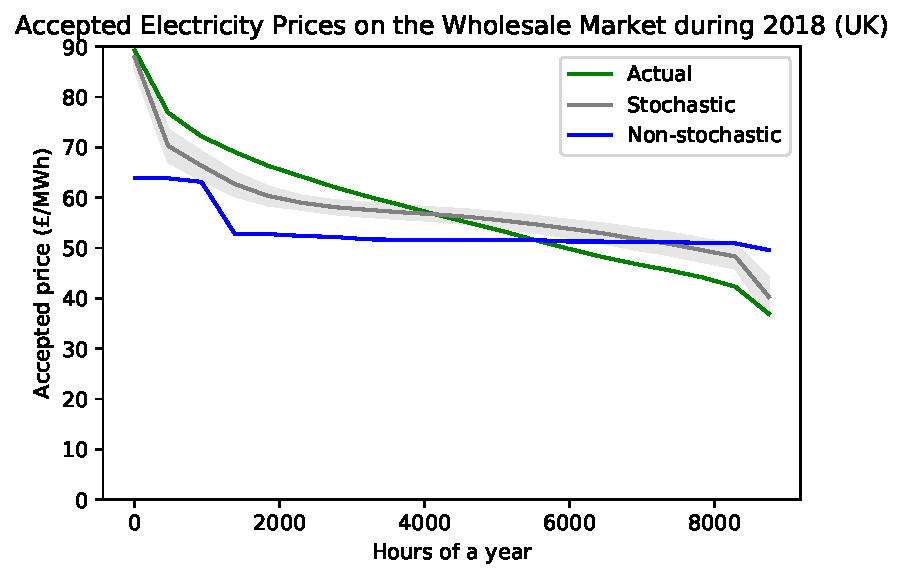
\includegraphics[width=0.5\textwidth]{figures/load_price_duration_curve_comparison.pdf}
		\caption{Price duration curve which compares real electricity prices to those paid in ElecSIM with stochasticity (40 runs) and no stochasticity.}
		\label{fig:price_duration_curve}
	\end{center}
\end{figure}

\begin{table}[h]
	\centering
	\csvautobooktabular{tables/validation/initialisation_run_validation.csv}
	\caption{Validation performance metrics.}
	\label{table:validation_metrics}
\end{table}

\subsection{Performance and Implementation}

ElecSIM was built using python, this enabled us to lower barriers to entry and allow for users to integrate state-of-the-art machine learning and statistical packages in future work. We used project mesa as an open source agent based modelling framework for its ease of use \cite{Masad2015}.

 We utilised Microsoft Azure Public Cloud. We used two virtual machines of 64 vCPU's each (D64 v3), which are built using Intel Broadwell E5-2673 v4 2.3GHz processor, and the Intel Haswell 2.4 GHz E5-2673 v3. They have a combined total of 256GB of memory and use a Linux operating system. This enabled us to rapidly prototype different demand and carbon price scenarios, and produce multiple iterations to gain a variance.

Development and testing was done on a MacBook Pro with a quad-core 3.1GHz Intel Core i7 processor with 16 GB 1867 MHz DDR3 of RAM and a 500GB solid state drive (SSD).

\begin{itemize}
	\item Validation of model 
	\begin{itemize}
		\item Compare price duration curve
		\item Compare power plant costs and NPV calculations
		\item Look number of steps ahead to compare electricity mix and compare to actual (cross-validation)
	\end{itemize} 
	\item Performance metrics - Comparison with EMLab, PowerACE (15 minute run time)
	\begin{itemize}
		\item Memory, disk size, runtime
		\item Increase in time complexity with additional data.
	\end{itemize}
\end{itemize}
